%%%%%%%%%%%%%%%%%%%%%%%%%%%%%%%%%%%%%%%%%%%%%%%%%%%%%%%%%%%%%%%%%%%%%%%%%%%%%%%%%%%%%%%%%%%
%                               My System 24pp
%%%%%%%%%%%%%%%%%%%%%%%%%%%%%%%%%%%%%%%%%%%%%%%%%%%%%%%%%%%%%%%%%%%%%%%%%%%%%%%%%%%%%%%%%%%
\chapter{Prototype}
\label{sec:implementation}

\section*{Summary}
A SleeveAR prototype was built to meet our vision expectations. To implement all planned features, our prototype had to rely on some already existing devices, mainly for motion tracking and feedback sources. This chapter will being with a description of our architecture and its most notable implementation details




\begin{figure}[!t]
    \begin{center}
        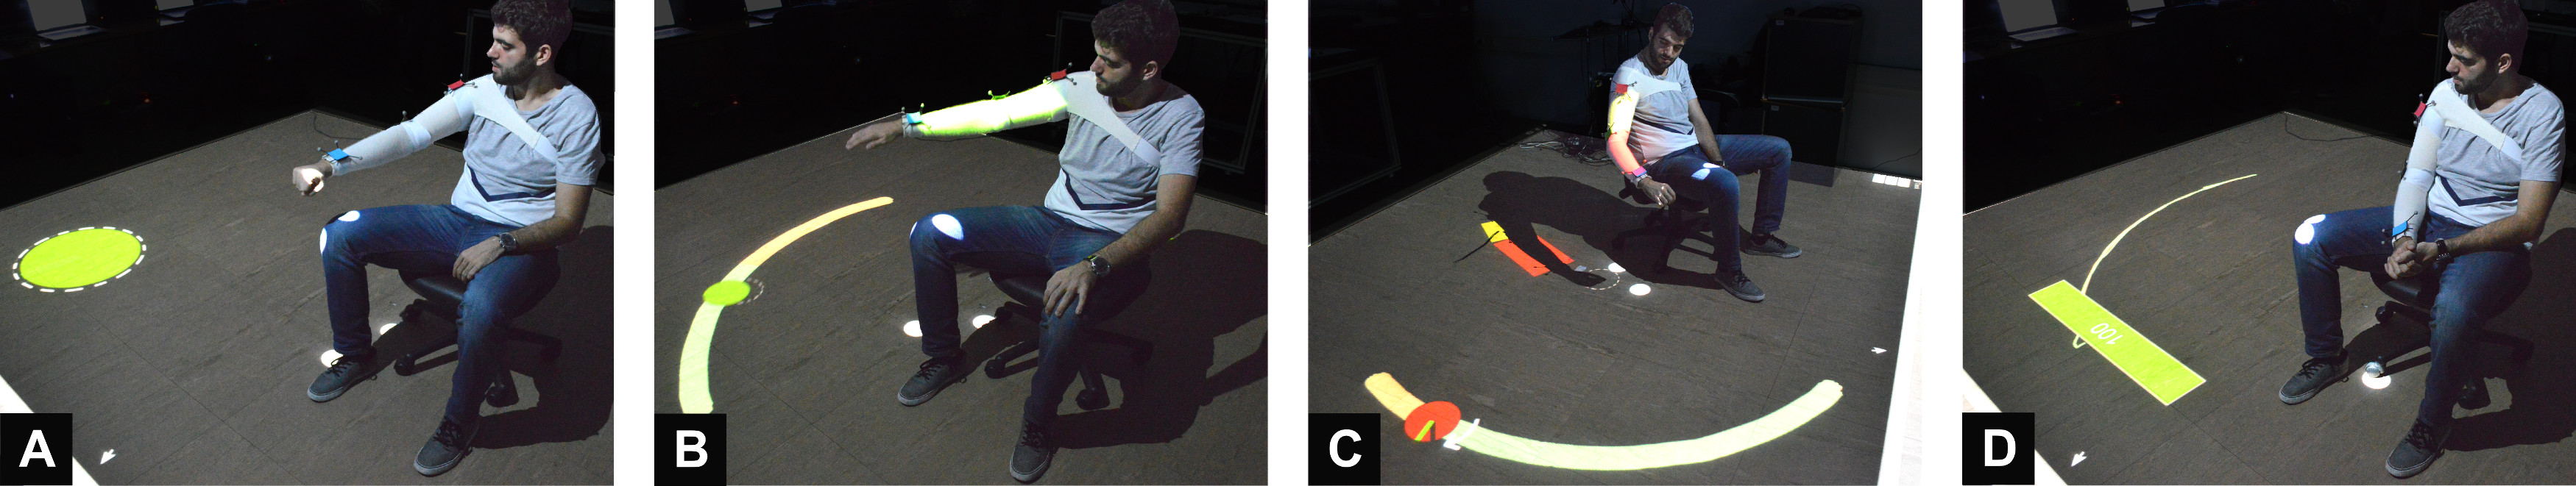
\includegraphics[width=\textwidth]{imgs/impl/teaser.jpg}
    \end{center}
    \caption{SleeveAR addresses new active projection-based strategies for providing user feedback during rehabilitation exercises. a) Initial position. b) Mid-performance. c) Sleeve Feedback. d) Performance review.}
    \label{fig:sleevewearable}
\end{figure}

\section{Architecture}
\label{sec:impl:arch}



\section{Tools}
\label{sec:impl:tools}

\subsection{Tracking Devices}


As for tracking devices, we had two different options to choose from.
The first makes use of the recently released, Microsoft Kinect One\footnote{\url{http://www.xbox.com/xboxone/kinect}} 
(previously baptized as Kinect 2), which supposedly offers a better tracking quality than 
the previous version, Kinect 1. Although this might be true, for our implementation we wanted a much more accurate and faster source of tracking, while also with a not so common tendency to fail due to camera occlusion.

The other alternative available at our laboratories was an OptiTrack Motion Capture system \footnote{\url{https://www.naturalpoint.com/optitrack/}}. 
This option offered us a more precise tracking and the possibility of dealing with occlusions due to the multiple cameras scattered around the room. 
The downside is the fact that it requires body markers to be used in order to successfully detect a person, unlike the 
Kinect which detects the human body through software algorithms. 
But using a comfortable and rather easy way to attach these body markers, made this not a bigger issue as it seems. 
A description of how we used the body markers can be found in section \ref{prototype-tracking}.



\subsection{Feedback Devices}

Providing feedback could be considered one of the foundations of this work. 
We chose to provide both visual and auditory feedback, being the latter much less vital to our goals in this implementation.

As it was described in section \ref{sec:sleevear}, our planned visual feedback would be applied on the user's arm and floor.
We relied on a light projector attached to the ceiling of our laboratory to project all visual feedback.
Details about how the light projections were able to hit the correct places, specifically the user's moving arm and floor, will be explained in section \ref{prototype-projection}.

Audio feedback was used simply to notify the user when to start the exercise and \todo{COMPLETAR}.
To provide audio, we relied on a speaker system also available at our laboratory

\subsection{Software}

We chose to implement our prototype with the well known \emph{Unity3D} game engine\footnote{\url{http://www.unity3d.com}}.
This engine already provides several tools that facilitate the development of augmented reality applications and we have in our possession already developed frameworks to communicate with the available tracking devices. In addition to this, Unity3D uses \texttt{C\#} as his main programming language, which is one of the most common languages use in the game development world, and already offers a wide range of solutions to create visual information.

\section{Setup Environment}
\todo{foto da sala}

\begin{figure}[!t]
\centering
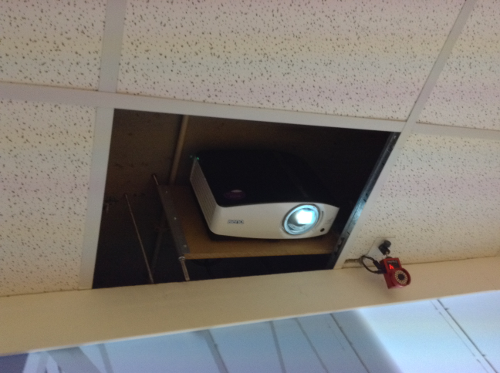
\includegraphics[width=0.5\textwidth]{imgs/impl/projector.png}
\caption{Light Projector}
\label{fig:projector}
\end{figure}

All the work here presented was conducted in the Jo\~ao Louren\c{c}o Fernandes Laboratory, located at Campus Taguspark of T\'ecnico Lisboa, seen at figure \todo{figura}.
In this laboratory we had at our disposal all required devices to implement our work.

There were Optitrack motion sensors already fixed on the walls and prepared to use UDP communication to send tracking data. 
In section \ref{prototype-tracking} we will further explain the key points about our tracking system.

The light projector is a short-throw Benq MP780 ST+, attached to the ceiling, as seen in figure \ref{fig:projector}, and
was used by connecting a VGA cable to our working computer. We used a resolution of \textit{1280x1024} which resulted in a floor projection of approximately \textit{4.3x3.3} 
meters.

\section{Implementation}

\subsection{Tracking}
\label{prototype-tracking}

\begin{figure}
\minipage[t]{0.32\textwidth}
  \centering
  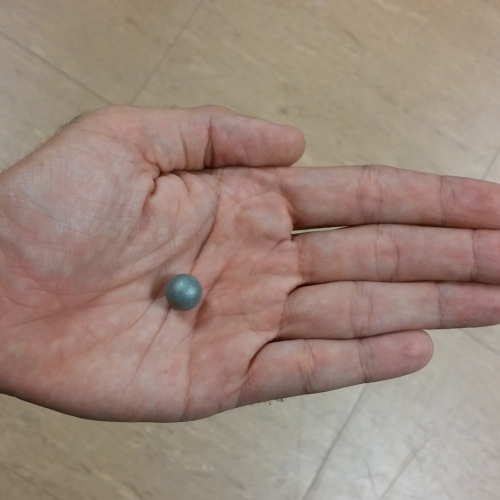
\includegraphics[width=\linewidth]{imgs/impl/singlemarker.png}
    \caption{Single Tracking Marker.}
    \label{fig:singlemarker}
    \endminipage\hfill
\minipage[t]{0.32\textwidth}
  \centering
  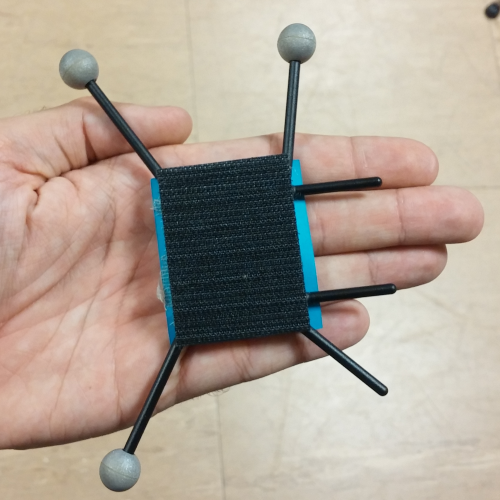
\includegraphics[width=\linewidth]{imgs/impl/markercombination.png}
    \caption{Marker Combination.}
    \label{fig:markercombination}
    \endminipage\hfill
\minipage[t]{0.32\textwidth}
  \centering
  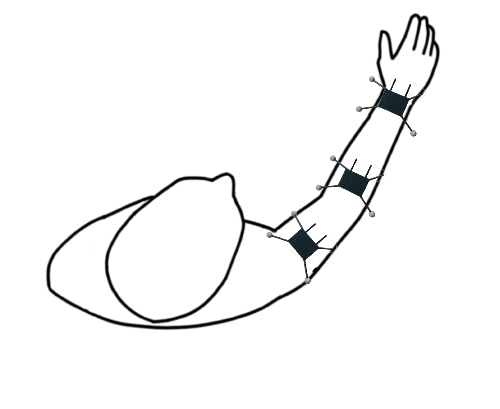
\includegraphics[width=\linewidth]{imgs/impl/rigidbodiesattached.png}
    \caption{Markers location on arm.}
    \label{fig:rigidbodiesattached}
    \endminipage
\end{figure}


As previously stated, we chose the Optitrack as our tracking system to implement SleeveAR's approach. This tracking system relies on body markers to capture movement.
These body markers are made of reflective material and are usually shaped as small spheres as we can see in figure \ref{fig:singlemarker}.
But Optitrack is not able to track one single marker, instead, we need to use combinations of markers for it to calculate both 
position and rotation of the combination's center of mass. 
To create combinations, we used small plastic objects onto which was possible to attach several markers exactly as the one being shown in figure \ref{fig:markercombination}.

After combining at least three markers, they could be assigned an ID inside Optitrack software. 
From then on, the software was able to identify that specific combination and provide us with its current position and rotation.
For easier understanding, and writing, of this section, we will name this markers combination as a \textbf{rigid body}.

With this in mind, for our work, we required three different rigid bodies. Each one should be attached to a different arm location, in this case, shoulder, elbow and wrist. 
By doing so, we were able to receive tracking data from the three locations, and therefore, replicate the arm with data. In figure \ref{fig:rigidbodiesattached} we can observe
an approximate location of each rigid body.

Our first method of placing the each rigid body was by using a Velcro bracelet around each location of the arm. 
Each rigid body would then be attached to each bracelet. This method didn't have a positive result for several reasons. 
First, it took to long to attach each bracelet around the arm, in addition, the Velcro material provoked discomfort when pressed hard against the skin. 
Second, the bracelets tended to move out of place, especially in the shoulder area where it was particularly hard to properly hold it in place.

Having an easy way to attach and hard to move method of holding our rigid bodies was vital for our work. 
Rigid bodies moving out of place during a movement could result in unwanted and unexpected results. 
Therefore, we created a better attachment method, by using a custom designed sleeve.

%\subsubsection{Sleeve}

\begin{figure}[!t]
    \begin{center}
        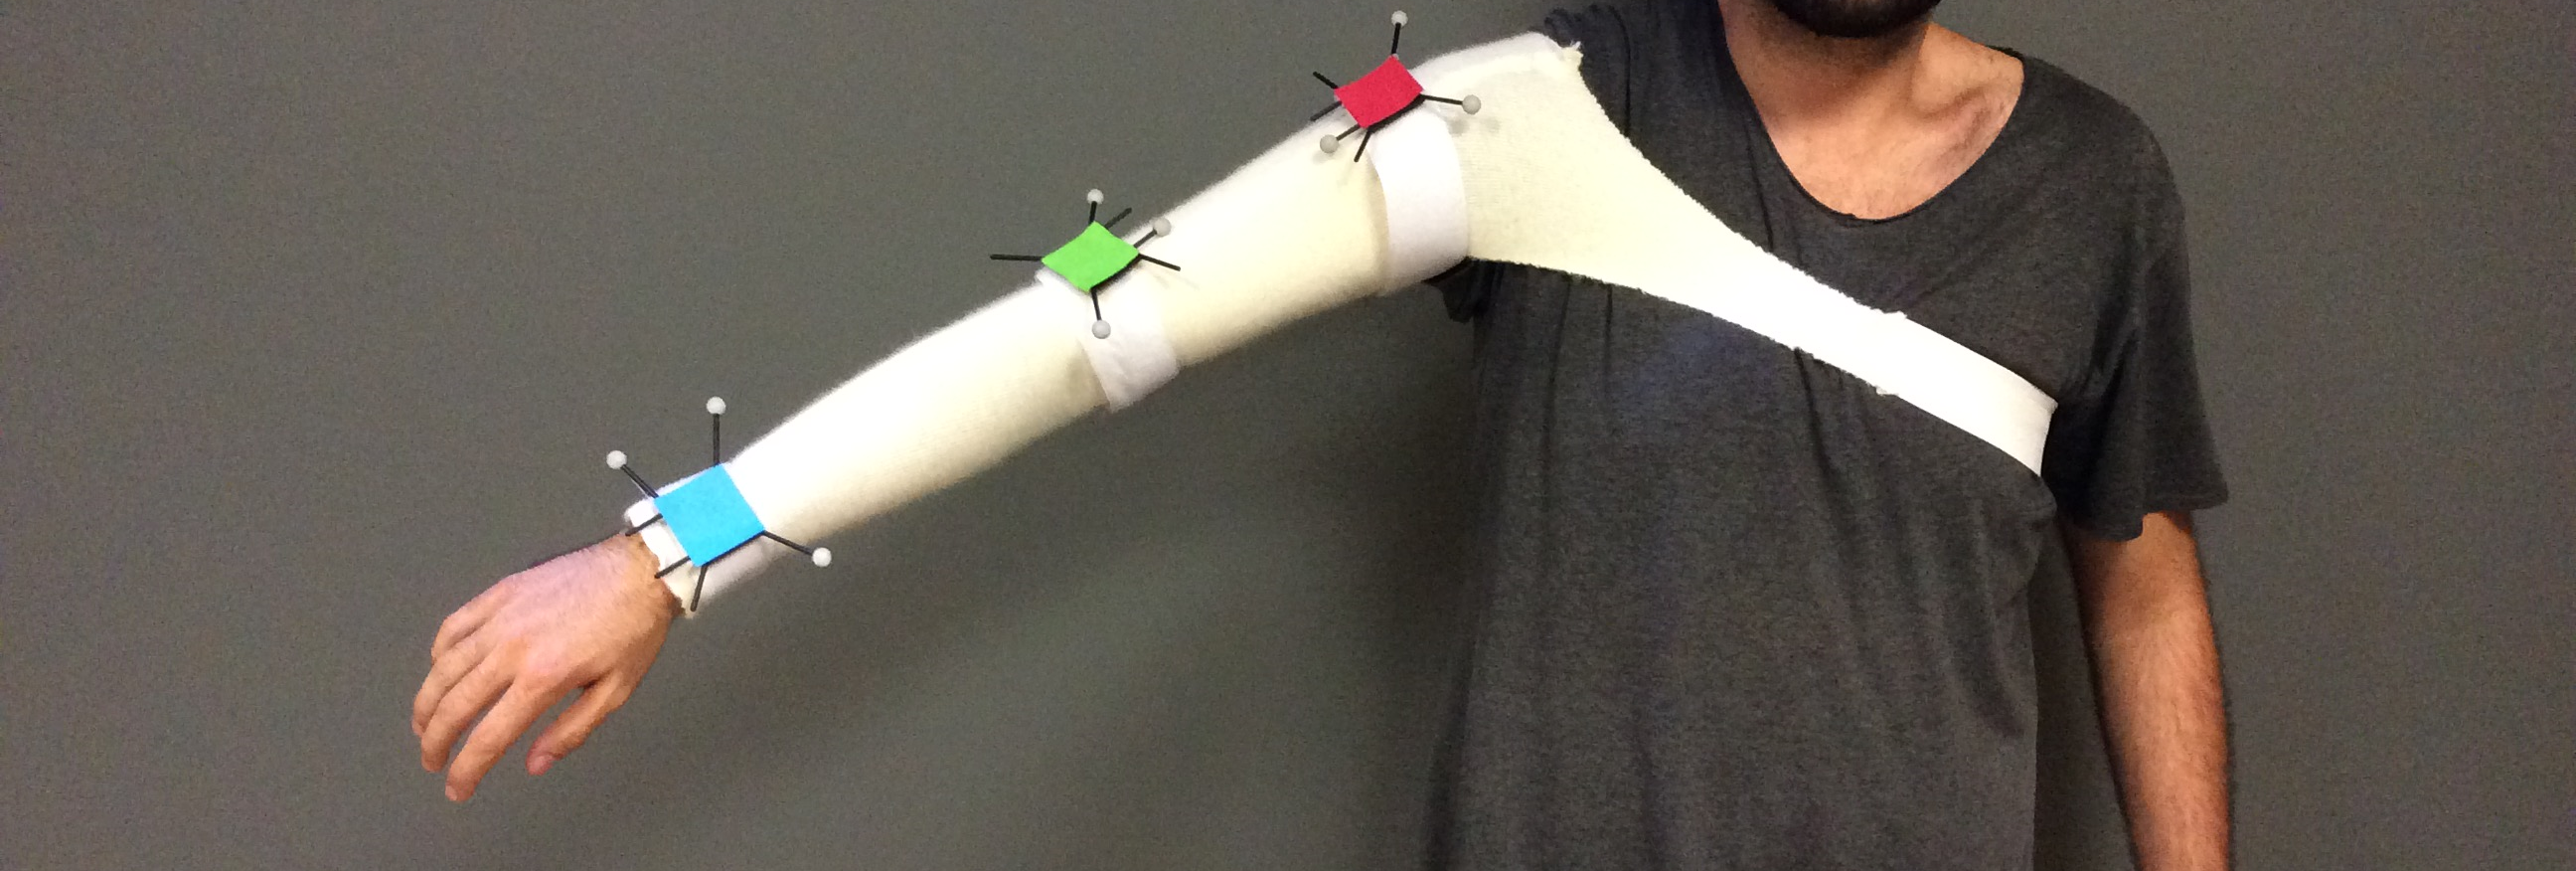
\includegraphics[width=\textwidth]{imgs/impl/sleevewearable.png}
    \end{center}
    \caption{Sleeve used for tracking.}
    \label{fig:sleevewearable}
\end{figure}

We designed a custom sleeve, seen at figure \ref{fig:sleevewearable}, made out of wool material. 
This solved our previously presented problems by fixing the sleeve in place using a kind of "belt" around the user's torso which greatly increased its stability. 
Each of the rigid bodies were still attached to a bracelet, but in this case the bracelets were stitched to the sleeve. 
This improved significantly the rigid bodies attachment due to the bracelets never leaving the sleeve, 
while also enabling us to still squeeze them more or less depending on the user's arm thickness.

\todo{white because of the color projections}

\subsection{Projection}
\label{prototype-projection}

\todo{explicar tecnica de projection no chao e braco}

\subsection{Recording Movements}

As it was described in section \ref{sec:sleevear:approach}, our prototype should be able to record demonstrated exercises for further use.
We implemented a simple interface to facilitate the recording process.

Assuming the user is already wearing our tracking sleeve, the \textbf{record} button, seen at figure \todo{picture interface learning}, simply had to be pressed to enable recording. 
After being pressed, an audio countdown was played through the laboratory speakers, in order to give the user some time to place himself in the desired exercise initial position. 
By standard, the recording time was set to a maximum duration of ten seconds, while capturing the arm tracking data 24 times per second.
The user could also stop the recording earlier if the exercise was not intended to take 10 seconds. He simply had to press the stop button.

Immediately after finishing recording, new options appear in the interface. 
The user could fill a text area with the intended file name and save the exercise, or first attach some more information to the file which we will explain next.

As we shown previously in section \ref{sec:movementguidance}, visual feedback provided during a movement included drawing the movement path on the floor. 
But this could become confusing if, for example, the recorded movement passed by the same place two times. 
The drawn path would intersect with itself, creating an unclear clue to where the movement might go next for the user. 
To avoid this, we implemented the \textbf{exercise parts}, which basically allowed us to divide the exercise in different parts and, consequently, divide also the drawn trajectory generated by our prototype.

To divide an exercise in parts, a slider was available in our interface which, when dragged, allowed to replay back and forth the recorded exercise. 
If the "Add Part" button was pressed, a division would be created in the the exercise based on where the slider currently was positioned.
All of this information was saved along with the exercises and stored on our computer.



\subsection{Data Storage}

Our stored files contained a list of all captured data from the three rigid bodies, as described in \ref{prototype-tracking}. 
Each of the list entries contained the position and rotation from each rigid body and also the required information to identify the different exercise parts in case they were assigned. 
If not, the exercises would be treated as one full movement without division.

We chose to save our information in the JSON format as oppose to XML due to generating much smaller file sizes. In addition to that, is was also a much more readable format, something we found useful when implementing and debugging this part of our prototype.

\subsection{Guiding}

\todo{figura feedback implementado}

Guiding a user through a recorded exercise, the core of our work, involved several phases for it to be possible.

First of all, we needed to load exercise files for them to be used again. 
We decided to use an already existing library, FullSerializer\footnote{\url{https://github.com/jacobdufault/fullserializer}}, for the sole purpose of reading and parsing JSON files.
After loading an exercise file, we could then start guiding a user whenever we wanted.

To implement the planned visual feedback, described in section \ref{vision-feedback}, and for it to dynamically change throughout a movement, 
we divided responsibilities into two main components. We will refer to these components as services, more specifically, the \ac{FS} and \ac{ES}.
The \ac{FS} has the responsibility of manipulating the provided feedback while the \ac{ES} was responsible in deciding if the user was executing correctly the exercise.

In other words, considering an exercise as a list of specific arm directions that we want another person to replicate in the correct orders. 
Obviously, the exercise should start in the first entry of this list. 
Once the user gets close enough to these specific entry, the \ac{ES} will then advance to the next entry. 
This will keep happening until we reach the end of the list and the exercise is over.

With this in mind, every time \ac{ES} is focused on a specific entry, the information inside it will generate the so called visual feedback \textbf{desired state}. 
Therefore, grabbing the concept of current and desired state from section \ref{vision-feedback}, two things will happen. 
First, \ac{FS} will update the current state based on real-time tracking from our current user. 
Second, the desired state will be updated accordingly to the current entry \ac{ES} is focusing on.

Even though we were tracking rigid bodies positions, we could not blindly compare positions between the original and attempt.
As explained in section \ref{sec:skeletoncomparison}, the person which recorded an exercise could have, for example, a different arm length.
With this in mind, even though we were storing rigid bodies positions, we generated normalized vectors to represent the arm direction. 
Upper arm direction was a normalized vector pointing from should to elbow position, while the fore arm direction was a vector from elbow to wrist.
By comparing both arm region directions, we eliminate the physical differences between different user's arm.

\todo{JV:should I have a more low-level explanation of this? I wanted it to be "simple"}
\todo{JV:talk about thresholds?}

\subsection{Performance Review}

\todo{figura performance review}

Every time an exercise was finished, our prototype should present the user with a review of his attempt. 
As described in our approach, the review should contain trajectory comparison between the original exercise and user's attempt.
As for the score, we implemented a simple formula to return a value from 0 to 100. 
Unfortunately, only after finishing our user tests we discovered a better alternative, which we ended up using for our result analysis, in section \ref{sec:results}.
A picture of our performance review implementation can be seen in figure \todo{figura performance review}
